\documentclass{beamer}
\usepackage{beamerthemeshadow}
\usepackage{verbatim}

\usepackage{lastpage}
\usepackage{xcolor}
\usepackage{pgf}
\usepackage{colortbl}
\usepackage{hyperref}

\newcommand{\bi}{\begin{itemize}}
\newcommand{\ei}{\end{itemize}}
\newcommand{\be}{\begin{enumerate}}
\newcommand{\ee}{\end{enumerate}}
\newcommand{\bd}{\begin{description}}
\newcommand{\ed}{\end{description}}
\newcommand{\prbf}[1]{\textbf{#1}}
\newcommand{\prit}[1]{\textit{#1}}
\newcommand{\beq}{\begin{equation}}
\newcommand{\eeq}{\end{equation}}
\newcommand{\bdm}{\begin{displaymath}}
\newcommand{\edm}{\end{displaymath}}

\newcommand{\ft}[1]{
  \frametitle{\begin{tabular}{p{4.2in}r} \textcolor{white}{#1} & \small{\insertframenumber / \inserttotalframenumber} \end{tabular}}
  %\frametitle{\begin{tabular}{p{4.2in}r} \textcolor{white}{#1} & \small{\insertframenumber / 7} \end{tabular}}
  \setbeamercovered{transparent=18}
}

\newcommand{\eft}[1]{
  \frametitle{\begin{tabular}{p{4in}r} \textcolor{white}{#1} & \small{\hyperlink{f:questions}{\beamergotobutton{GO BACK}}} \end{tabular}}
  \setbeamercovered{transparent=18}
}

\newcommand{\stepinv}{\setbeamercovered{invisible}}
\newcommand{\stopinv}{\setbeamercovered{transparent=18}}
\newcommand{\uncoverinv}[1]
{
  \setbeamercovered{invisible}
  \uncover<+->{#1}
  \setbeamercovered{transparent=18}
}
\newcommand{\ans}[1]{\textcolor{blue}{#1}}
\newcommand{\ansinv}[1]
{
  \setbeamercovered{invisible}
  \uncover<+->{\textcolor{blue}{#1}}
  \setbeamercovered{transparent=18}
}
\newcommand{\setinv}{\setbeamercovered{invisible}}
\newcommand{\setvis}{\setbeamercovered{transparent=18}}
\newcommand{\centerpic}[2]
{
  \begin{center}
  \includegraphics[#1]{#2}
  \end{center}
}
\newcommand{\h}[1]{\hat{#1}}
\newcommand{\ds}{\displaystyle}

%\definecolor{light}{rgb}{1.0,0.33,0.33}
\definecolor{light}{rgb}{1.0,0.5,0.5}
\newcommand{\hl}[1]{\alt<#1>{\rowcolor{light}\hspace*{-2.1pt}} {\hspace*{-2.1pt}} }

\definecolor{mycolor}{rgb}{0.6,0.0,0.0}
\usecolortheme[named=mycolor]{structure}

\title{A Life Insurance Deterrent to Risky Behavior in Africa}
\author[James Murray, University of Wisconsin - La Crosse]{Pedro de Araujo\\Department of Economics and Business\\Colorado College\\ \and\\ James Murray\\Department of Economics\\University of Wisconsin - La Crosse}
\date{November 22, 2009}

\begin{document}

\frame{\titlepage \setcounter{framenumber}{0}}

\section{AIDS Epidemic}
\subsection{Introduction}
\frame
{
  \ft{AIDS Epidemic}
  \bi
  \item<+-> AIDS killed an estimated 2.1 million people worldwide in 2007.
  \item<+-> Between 30.6 and 36.1 million people worldwide currently live with HIV.
  \item<+-> About 2/3 of these people live in Sub-Saharan Africa.
  \item<+-> Worldwide, between 1.8 and 4.1 million new people become infected every year.
  \ei
}

\subsection{HIV/AIDS Prevention Campaigns}
\frame
{
  \ft{HIV/AIDS Prevention Campaigns}
  \bi
  \item<+-> HIV/AIDS funding was around \$10 billion in 2007.  
    \bi
    \item<.-> Almost a 40 fold increase from the previous 10 years.
    \ei
  \item<+-> Thailand and Cambodia: successful prevention campaigns focused on commercial sex workers.
    \bi
    \item<.-> Led to a 90\% increase in condom use and 50\% reduction in demand.
    \ei
  \item<+-> Longer-term relationships: 
    \bi
    \item<.-> Ku, Sonenstein, and Pleck (1994): condom use declines with age and length of relationship.
    \ei
  \ei
}

\subsection{Reasons for Risky Behavior}
\frame
{
  \ft{Reasons for Risky Behavior}
  \bi
  \item Oster (2007): risky sexual behavior is greater for those with
    \bi
    \item<+-> shorter life expectancies,
    \item<+-> smaller life time incomes.
    \item<+-> Find decisions of heterosexual males in Sub-Saharan Africa are consistent with homosexual males in United States.
    \ei
  \item<+-> Becker (1993): Education may increase lifetime income and decrease risky behavior.
  \item<+-> Grossman (1972) and Kenkel (1991): Education may increase access to health information and facilities.
  \item<+-> Can life insurance (paid only if HIV negative) also replicate higher life expectancy and higher lifetime income?
  \ei
}

\section{Model}
\subsection{Overview}
\frame
{
  \ft{Model Overview}
  \bi
  \item<+-> Model the behavior of adult males with dependents.
  \item<+-> Derive utility and make decisions about:
    \be
    \item<+-> Personal consumption.
    \item<+-> Family consumption.
    \item<+-> Number of risky sexual partners.
    \ee
  \item<+-> Three period model:\newline~~~~ 1) Ages 25-39~~ 2) Ages 40-54~~ 3) Ages 55-69
  \item<+-> Agents alive in period 1, possibly die before periods 2 and 3.
    \bi
    \item<+-> Exogenous factors with probability $\delta \in (0,1)$
    \item<+-> Contracting HIV in period $t$, die of AIDS between $t$ and $t+1$.
    \ei
  \ei
}

\frame
{
  \ft{Preferences}
  Period $t \in \{1,2,3\}$ utility function:
  \uncover<+->{\bdm u(c_t, f_t, m_t) = v(c_t, f_t) + \gamma_t w(m_t) \edm}
  \vspace*{-1pc}
  \bi
  \item<+-> $c_t$: personal consumption
  \item<+-> $f_t$: family consumption
  \item<+-> $m_t$: number of sexual partners
  \item<+-> $\gamma_t$ measures relative preference for sexual partners.
  \ei
}

\frame
{
  \ft{Preference for Consumption}
  \uncover<+->{Log utility over CES personal/family consumption bundle:}\\
  \uncover<+->{\bdm \begin{array}{l} \ds v(c_t, f_t) = \\ \\
  \ds \log\left( \left[\alpha \left(c_t + \epsilon\right)^{\frac{\nu-1}{\nu}} + (1-\alpha) \left(f_t + \epsilon \right)^{\frac{\nu-1}{\nu}} \right]^{\frac{\nu}{\nu-1}} \right) - \log(\epsilon) \end{array} \edm}
  \bi
  \item<+-> $\alpha$: preference for personal vs family consumption.
  \item<+-> $\nu$: elasticity of substitution personal vs family consumption.
  \item<+-> Small value of $\epsilon$ forces $v(0,0)=0$.
  \item<+-> If husband is alive, $c_t, f_t > 0$, $v(c_t,f_t)>0$, $v_{c}(c_t,f_t)>0$ $v_{f}(c_t,f_t)>0$, $v_{cc}(c_t,f_t)<0$, $v_{ff}(c_t,f_t)<0$.
  \item<+-> If husband is dead, $c_t=0$ but $f_t>0$ and $v(0,f_t)>0$, $v_{f}(0,f_t)>0$, $v_{ff}(0,f_t)<0$.
  \ei
}

\frame
{
  \ft{Preference for Sexual Partners}
  \bi
  \item<+-> Assume no sexual partners in final period (ages 55-79).
  \item<+-> Increases in number of sexual partners increases utility...
  \item<+-> Until reach a satiation point $m^*$ where $w'(m^*) = 0$.
  \uncover<+->{\bdm w(m_t) = \log\left[-\left(m_t - m^*\right)^2 + \left(m^*\right)^2 + \epsilon\right] - \log(\epsilon) \edm}
  \vspace*{-0.5pc}
  \item<+-> Small value of $\epsilon$ forces $w(0)=0$ if agent is dead.
  \item<+-> If agent is alive and $m_t < m^*$, $w(m_t)>0$, $w'(m_t)>0$, $w''(m_t)<0$
  \item<+-> Inada condition $\ds \lim_{\epsilon\to 0} \lim_{m_t\to 0} w'(m_t,\epsilon) = \infty$ guarantees interior solution.
  \ei
}

\subsection{HIV Transmission}
\frame
{
  \ft{HIV Transmission}
  \bi
  \item<+-> Let $h \in (0,1)$ be the HIV prevalence among potential partners.
  \item<+-> Let $t \in (0,1)$ be the female-to-male transmission rate (per partnership).
  \item<+-> For a given partner, probability of not contracting HIV: $(1-ht)$.
  \item<+-> For $m_t$ partners: $(1-ht)^{m_t}$.
  \item<+-> Probability of contracting HIV in period $t$, die before $t+1$:
    \uncover<+->{\bdm \pi(m_t) = 1 - (1-ht)^{m_t} \edm}
    \uncover<+->{= HIV prevalence among age group $t$}
  \ei
}

\subsection{Optimization Problem}
\frame
{
  \ft{Expected Life-Cycle Utility}
  \uncover<+->{Expected utility over three periods:}
  \bdm \begin{array}{l} \uncover<+->{U = \ds u(c_1, f_1, m_1)} \uncover<+->{+ \beta (1-\delta)\left[1-\pi(m_1)\right] u(c_2, f_2, m_2)} \\\\ 
  \uncover<+->{\ds + \beta \left\{1 - (1-\delta)\left[1-\pi(m_1)\right] \right\} u(0,f_2,0)} \\ \\
  \uncover<+->{\ds + \beta^2 (1-\delta)^2 \left[1-\pi(m_1)\right]\left[1-\pi(m_2)\right] u(c_3, f_3, 0)} \\ \\
  \uncover<+->{\ds + \beta^2 \left\{1 - (1-\delta)^2 \left[1-\pi(m_1)\right]\left[1-\pi(m_2)\right]\right\} u(0, f_3, 0)} \end{array} \edm

  \only<1>{Each component of utility function:}
  \only<2>{Utility from everything in period 1 -- definitely alive.}
  \only<3>{(Utility from everything in period 2) x (Prob alive).}
  \only<4>{(Utility from only family cons in period 2) x (Prob dead).}
  \only<5>{(Utility from family/personal cons in period 3) x (Prob alive).}
  \only<6>{(Utility from only family cons in period 3) x (Prob alive).}
}

\frame
{
  \ft{Expected Life-Cycle Budget Constraint}
  \uncover<+->{Expected budget constraint over three periods:}
\bdm \begin{array}{l} \uncover<2->{\ds p_1(c_1 + f_1)} \uncover<3->{+ (1-\delta) \left[1-\pi(m_1)\right] \frac{p_2 c_2}{1+r}} \uncover<4->{+ \frac{p_2 f_2}{1+r} }\\ \\
\ds \uncover<5->{+ (1-\delta)^2 \left[1-\pi(m_1)\right] \left[1-\pi(m_2)\right] \frac{p_3 c_3}{\left(1+r\right)^2}} \uncover<6->{+ \frac{p_3 f_3}{\left(1+r\right)^2}} \\ \\
\ds \uncover<2->{= w_1} \uncover<3->{+ (1-\delta) \left[1-\pi(m_1)\right] \frac{w_2}{1+r}} \uncover<7->{+ \delta \left[1-\pi(m_1)\right] \frac{b_2}{1+r}} \\ \\
\ds \uncover<8->{+ \delta (1-\delta) \left[1-\pi(m_1)\right] \left[1-\pi(m_2)\right] \frac{b_3}{(1+r)^2}} \end{array} \edm

  \only<1>{Each component of budget constraint:}
  \only<2>{Income and personal and family cons period 1 -- definitely alive.}
  \only<3>{(Income and expenses from personal cons period 2) x (Prob alive).}
  \only<4>{Certain family consumption period 2.}
  \only<5>{(Expenses from personal cons period 3) x (Prob alive).}
  \only<6>{Certain expense on family consumption in period 3.}
  \only<7>{$b_2:$ Life insurance if dead in period 2, but not from HIV.}
  \only<8>{$b_3:$ Life insurance if alive in period 2, dead in 3, not from HIV.}
}

\section{Results}
\subsection{Parameters}
\frame
{
  \ft{Solving the Model}
  \bi
  \item<+-> The model has no closed form solution.
  \item<+-> For a given set of parameters, can use numerical methods and computing power.
  \item<+-> Simulate the model for a large range of parameters for...
    \bi
    \item<+-> life expectancy (influences $\delta$),
    \item<+-> income (assume $w_1=w_2$),
    \item<+-> size of life insurance benefit (assume $b_1=b_2$),
    \item<+-> elasticity of sub, $\nu$ (sensitivity analysis),
    \item<+-> preference for personal consumption, $\alpha$ (sensitivity analysis)
    \ei
  \ei
}

\frame
{
  \ft{Baseline Parameters}
  \bi
  \item<+-> HIV Prevalence among potential partners: $h = 0.119$.
  \item<+-> Transmission rate: $t=0.15$.
  \item<+-> Exogenous probability of dying: $\delta = 0.382$\\~~~ matches a 55 year life expectancy.
  \item<+-> Interest rate / Discount rate (15 year period):\\~~~ $r=0.82$, $\beta=0.547$.
  \item<+-> Income: $w_1=w_2=328.0$,\\ ~~~roughly real GDP per person Uganda (U.S. dollars).
  \item<+-> Prices: $p_1=p_2=p_3=1$.
  \item<+-> Life insurance: $b_2=b_3=0$
  \ei
}

\frame
{
  \ft{Baseline Preference Parameters}
  \bi
  \item<+-> Satiation point: $m^* = 50$.
  \item<+-> Personal consumption preference parameter: $\alpha=0.5$.
  \item<+-> Elasticity of sub personal/family consumption: $\nu=1.0$.
  \item<+-> Sexual partner preference parameters $\gamma_1 = 1.23$\\ ~~~(chosen to yield $\pi(m_1)=0.119$).
  \item<+-> Sexual partner preference parameters $\gamma_2 = 51$\\ ~~~(chosen to yield $\pi(m_2)=0.119$).
  \ei
}

\subsection{Dynamics of Risky Behavior}
\frame
{
  \ft{Response to Life Expectancy}
  \begin{center}
  \begin{tabular}{cc}
  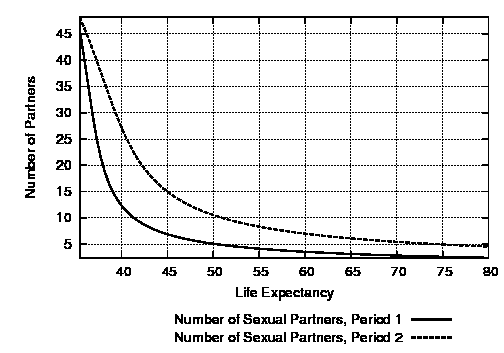
\includegraphics[scale=0.28]{mlife.png} & 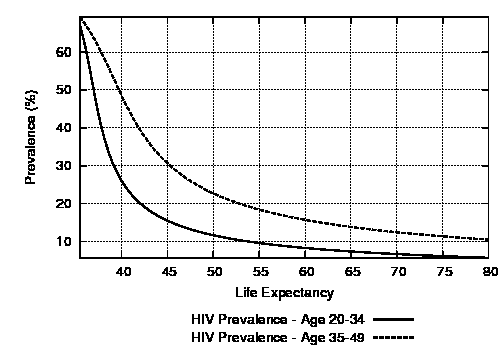
\includegraphics[scale=0.28]{hivlife.png} 
  \end{tabular}
  \end{center}
  \bi
  \item<+-> Choice for number of sexual partners decreases with life expectancy.
  \item<+-> HIV prevalence among adult men can decrease to about 7\% 
  \ei
}

\frame
{
  \ft{Response to Income}
  \begin{center}
  \begin{tabular}{cc}
  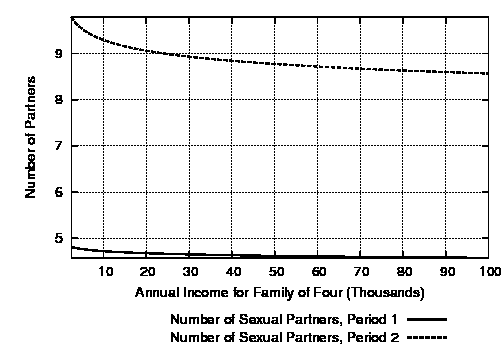
\includegraphics[scale=0.28]{mgdp.png} & 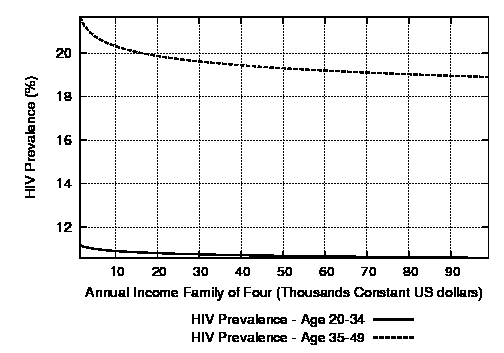
\includegraphics[scale=0.28]{hivgdp.png} 
  \end{tabular}
  \end{center}
  \bi
  \item<+-> Number of sexual partners decreases with income.
  \item<+-> HIV prevalence can decrease only to 10.9\% (young) and 10.1 (mid-age)\%. 
  \ei
}

\frame
{
  \ft{Responses to Life Expectancy and Income}
  \bi
  \item<+-> Smaller response to income than life expectancy.
  \item<+-> Possible higher income may never be earned (if die before period 2).
  \item<+-> For this reason, response is higher in period 2.
  \item<+-> Possible may not get to enjoy personal consumption with income.
  \item<+-> \textit{Combination} of high income and higher life expectancy should be larger...
  \ei
}

\frame
{
  \ft{Response to Life Expectancy and Income}
  \vspace*{-1pc}
  \begin{center}
    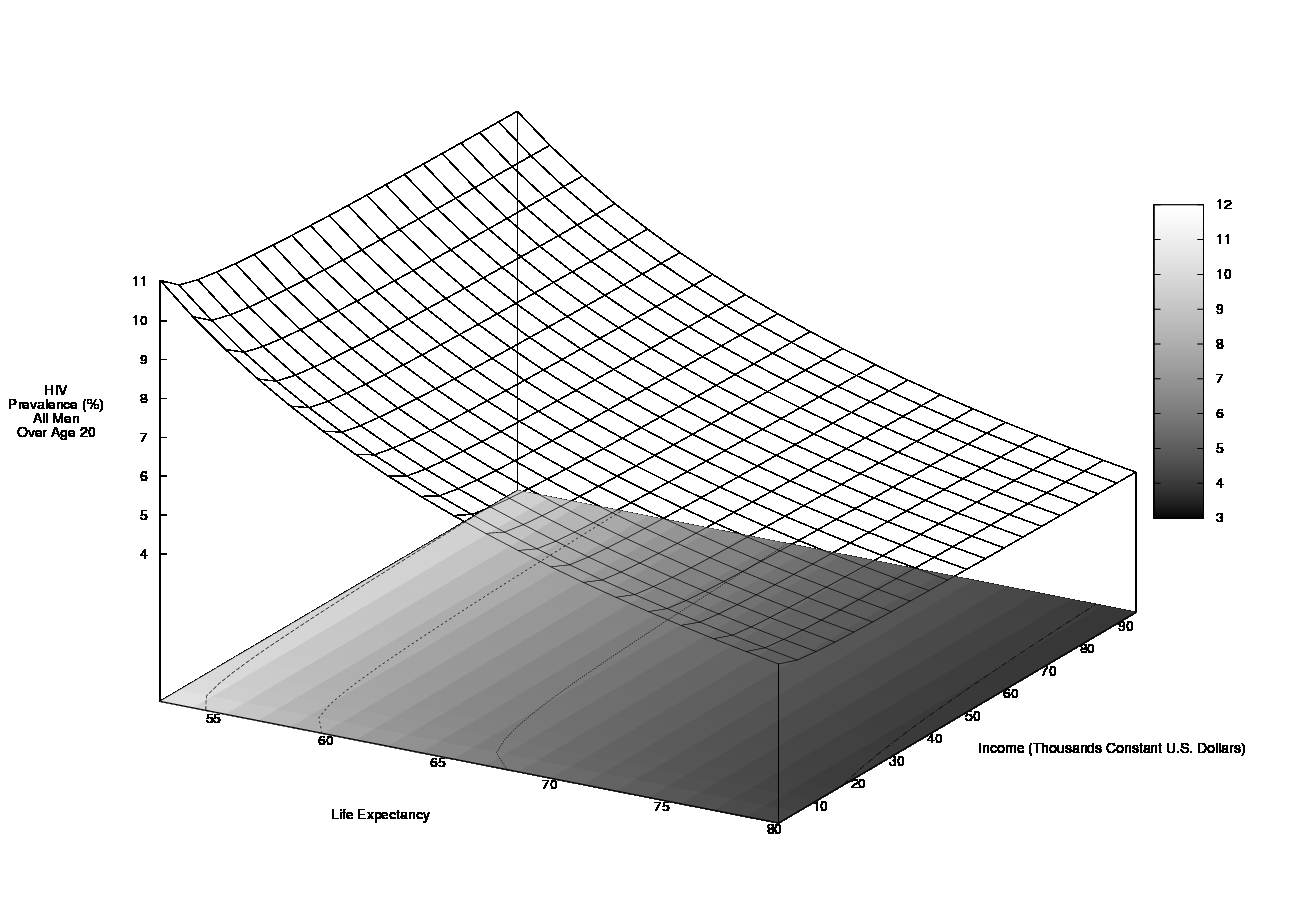
\includegraphics[scale=0.22]{hiv_gdplife.png}
  \end{center}
  Simultaneous increases in income and life expectancy can reduce HIV prevalence in adult males to about 4.5\%.
}

\frame
{
  \ft{Response to Life Insurance Benefit}
  \begin{center}
  \begin{tabular}{cc}
  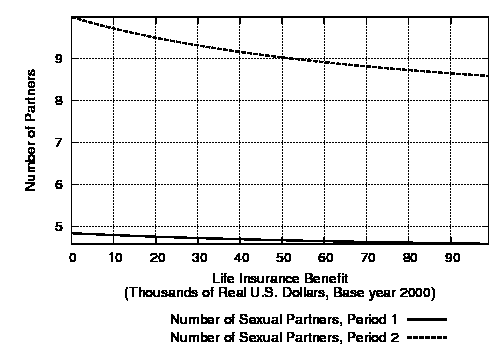
\includegraphics[scale=0.28]{mB.png} & 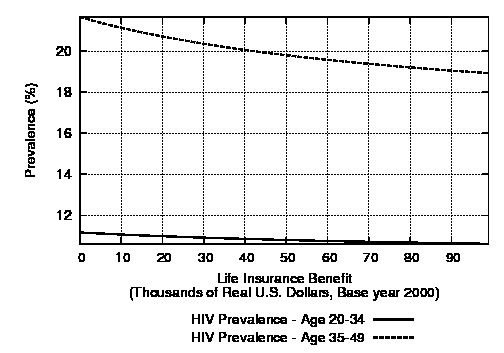
\includegraphics[scale=0.28]{hivB.png} 
  \end{tabular}
  \end{center}
  \bi
  \item<+-> Number of partners decreases with life insurance benefit.
  \item<+-> HIV decreases to 10.9\% (young) and 10.1\% (mid-age). 
  \item<+-> Largely mirrors the effect of an increase in income, not increase in life expectancy.
  \ei
}

\subsection{Parameter Sensitivity}
\frame
{
  \ft{Sensitivity: Preference Personal Consumption}
  \bi
  \item<+-> Choice for sexual partners depends on $\alpha$.
  \item<+-> Family income effect: lower $\alpha$ increases utility from family consumption.
    \bi
    \item<+-> Death causes a decrease in life-cycle expected income, lower family consumption.
    \item<+-> Causes one to decrease number of sexual partners.
    \item<+-> Only relevant in period 1.  If alive in period 2, already earned lifetime income.
    \ei
  \item<+-> Personal consumption effect: lower $\alpha$ decreases utility from personal consumption.
    \bi
    \item<+-> Death forces zero personal consumption, lower utility cost.
    \item<+-> Causes one to increase number of sexual partners.
    \item<+-> Relevant for periods 1 and 2.
    \ei
  \ei
}

\frame
{
  \ft{Sensitivity: Preference for Personal Consumption}
  \begin{center}
  \begin{tabular}{cc}
  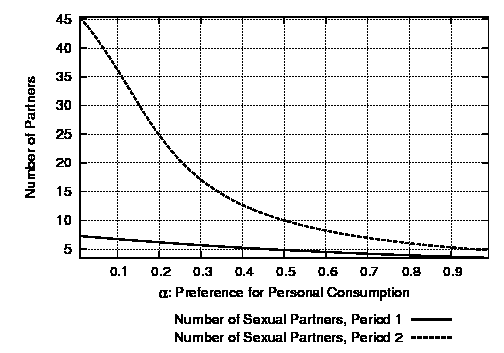
\includegraphics[scale=0.28]{malpha.png} & 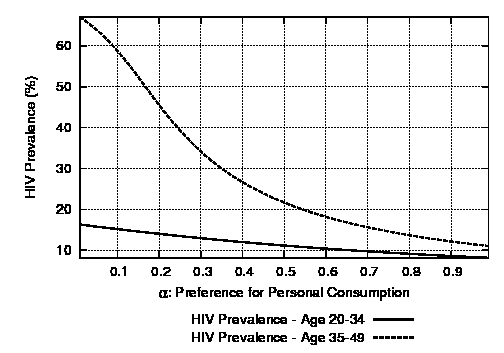
\includegraphics[scale=0.28]{hivalpha.png} 
  \end{tabular}
  \end{center}
  Increases in personal consumption preference causes a \textit{decrease} in sexual partners.
}

\frame
{
  \ft{Life Insurance: Preference for Personal Consumption}
  \bi
  \item<+-> How does influence of life insurance on sexual behavior depend on $\alpha$?
  \item<+-> Simulate model for values of $\alpha$ between 0, 1.
  \item<+-> For each value of $\alpha$, pick $\gamma_1$ and $\gamma_2$ so that $\pi(m_1)=\pi(m_2)=0.119$.
  \item<+-> For each value of $\alpha$, simulate model for various life insurance benefits.
  \ei
}

\frame
{
  \ft{Life Insurance: Personal Consumption}
  \vspace*{-1pc}
  \begin{center}
    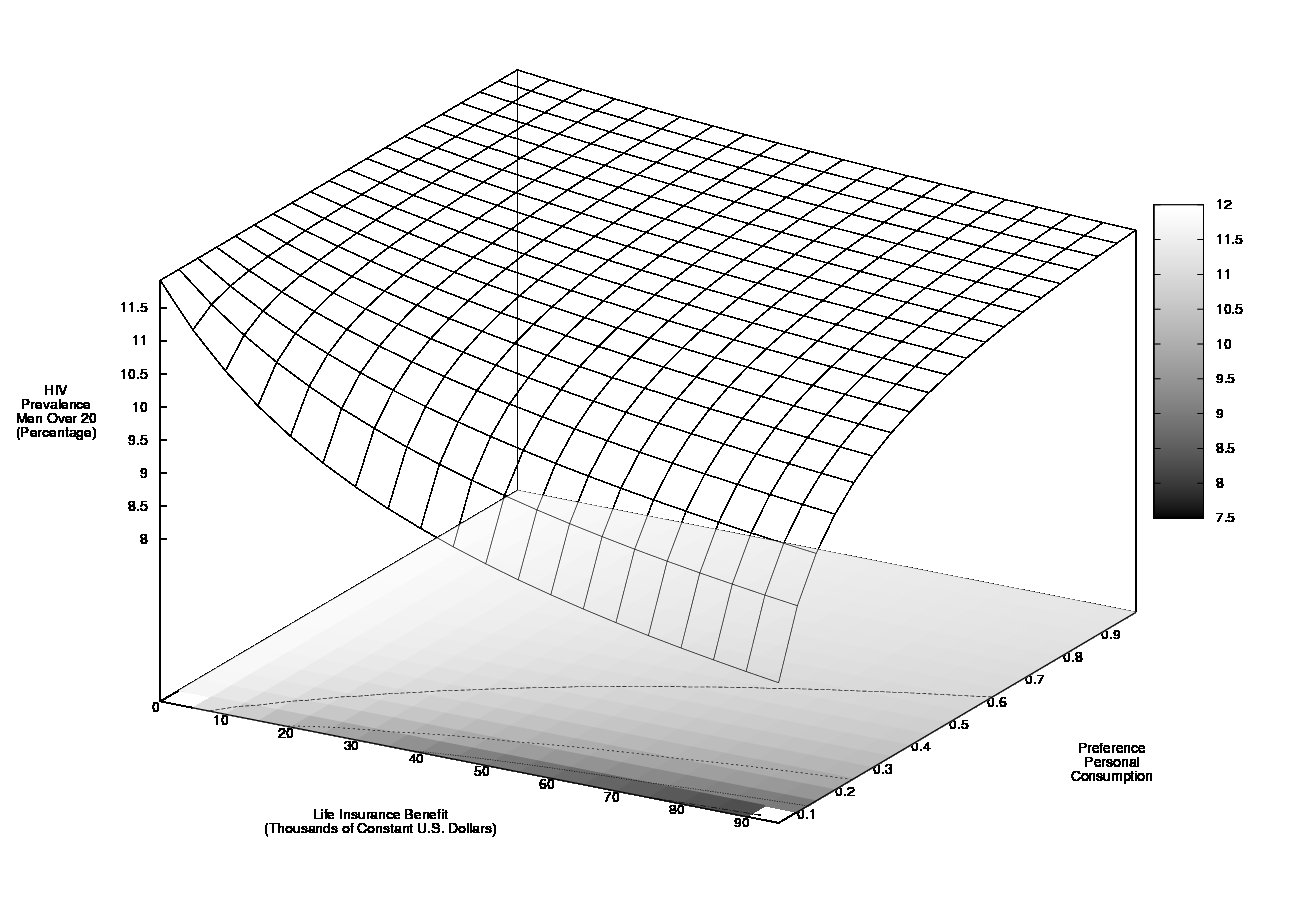
\includegraphics[scale=0.22]{hivBalpha.png}
  \end{center}
  Decrease in preference for personal consumption causes an \textit{increase} in effectiveness.
}

\frame
{
  \ft{Sensitivity: Elasticity of Substitution}
  Family substitution effect:
    \bi
    \item<+-> Suppose personal and family consumption are highly substitutable (high $\nu$).
    \item<+-> Consequence of dying from AIDS: low impact on utility from $c_t=0$.
    \item<+-> Choose more sexual partners.
    \ei
}

\frame
{
  \ft{Sensitivity: Elasticity of Substitution}
  \begin{center}
  \begin{tabular}{cc}
  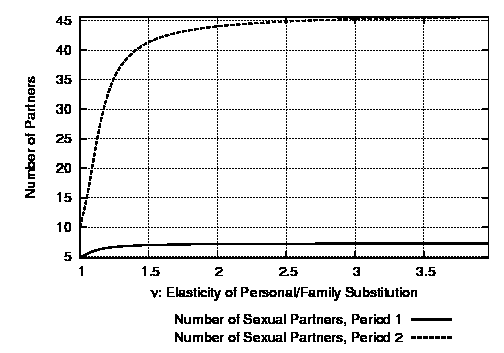
\includegraphics[scale=0.28]{msub.png} & 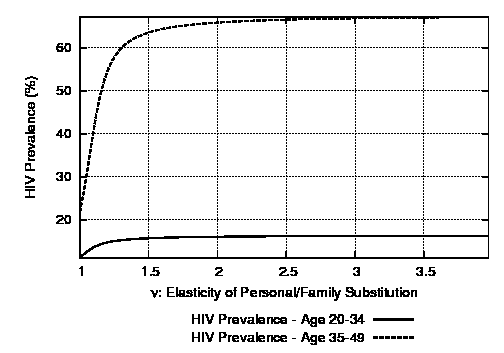
\includegraphics[scale=0.28]{hivsub.png} 
  \end{tabular}
  \end{center}
  Increases in elasticity of substitution causes an \textit{increase} in sexual partners.
}

\frame
{
  \ft{Life Insurance: Elasticity of Substitution}
  \vspace*{-1pc}
  \begin{center}
    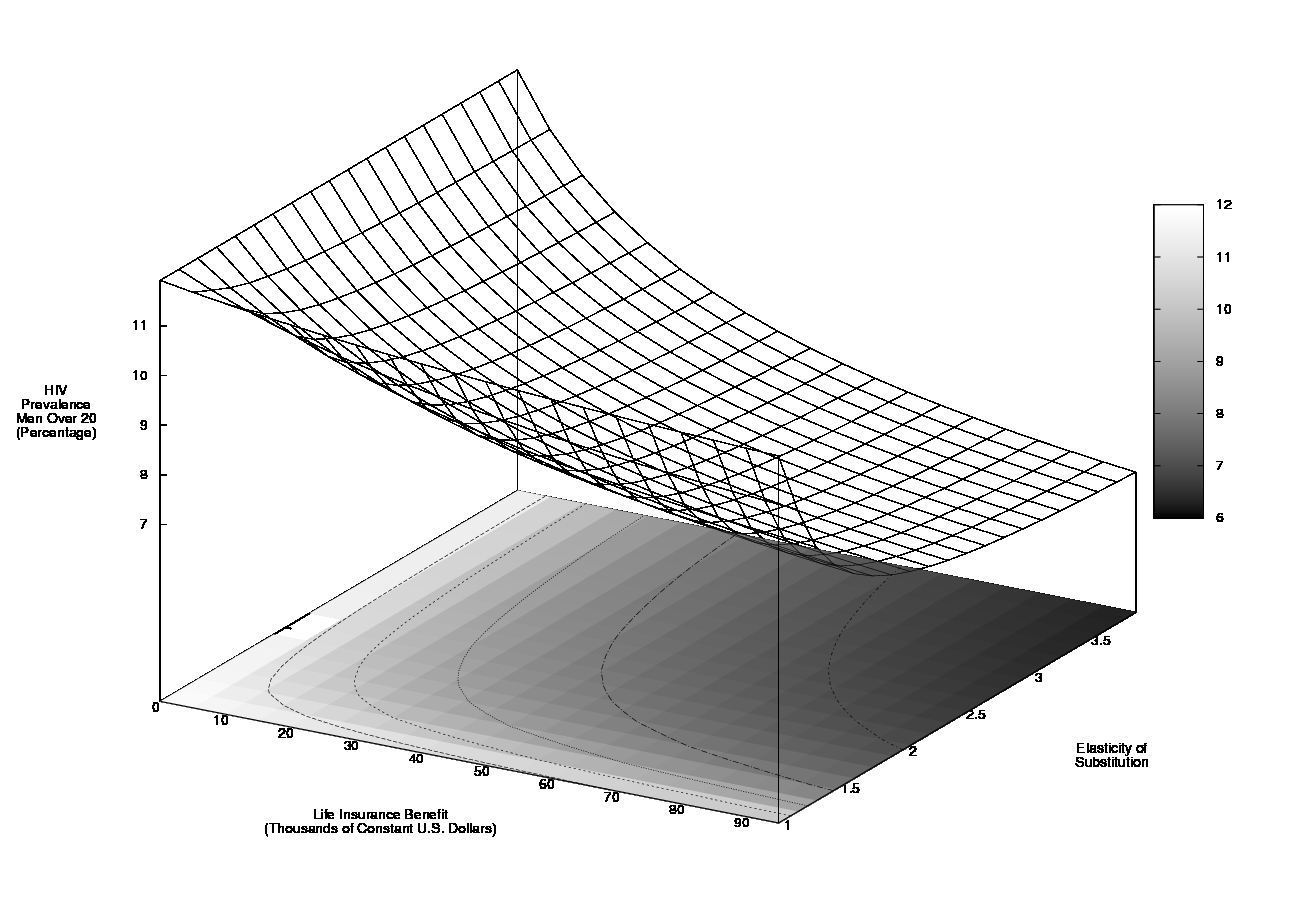
\includegraphics[scale=0.22]{hivBsub.png}
  \end{center}
  Increases in elasticity of substitution causes an \textit{increase} in effectiveness.
}

\frame
{
  \ft{Life Insurance: Elasticity of Substitution}
  \bi
  \item<+-> Increase in substitutability increases number of sexual partners (\textit{ceteris paribus}).
  \item<+-> Increase in substitutability increases life insurance deterrence.
  \item<+-> Life insurance has greater ability to mimic high life expectancy.
    \bi
    \item<+-> If dead, family consumption acts as a suitable substitute for personal consumption.
    \item<+-> Little utility cost to lost personal consumption.
    \item<+-> Increases income over life-cycle.
    \ei
  \item<+-> Life insurance can decrease HIV prevalence to about 3.5\%.
  \ei
}

\section{}
\subsection{Conclusion}
\frame
{
  \ft{Conclusion}
  \bi
  \item<+-> Life-cycle model
    \bi
    \item<+-> Low life expectancy and low income leads to highly risky behavior.
    \item<+-> High life expectancy and high income leads to much safer behavior.
    \ei
  \item<+-> Life insurance can replicate small effects of a high income.
  \item<+-> Life insurance can replicate large effects of \textit{both} a high income and high life expectancy,
    \bi
    \item<+-> if value for personal consumption versus family consumption is low and/or
    \item<+-> if elasticity of substitution between personal and family consumption is high.
    \ei
  \item<+-> Easy for life insurance deterrent to have large coverage.
  \item<+-> Should encourage HIV testing, complement existing prevention measures.
  \ei
}


\end{document}

